\subsection{Minimal Service Model}
\label{subsec:minimal-service-model}

Minimal Service Model adalah sebuah RDF(S) Integration Ontology sederhana berdasarkan prinsip \textit{minimal ontological commitment}, yaitu prinsip dalam perancangan ontologi yang berarti membuat klaim atau asumsi sesedikit mungkin tentang domain yang dimodelkan. Visualisasi dari ontologi MSM dapat dilihat pada gambar \ref{image:msm-visualization}. MSM hanya mendefinisikan struktur dasar seperti Services, Operations, dan Message Content. MSM dikembangkan bukan untuk menambah keragaman model \textit{service} yang sudah ada, melainkan berfungsi sebagai model untuk integrasi yang menjembatani berbagai formalisme yang telah ada. Model ini mampu menangkap semantik inti dari Web Service dan Web API dalam satu model yang sama, sehingga mendukung proses publikasi dan penemuan \textit{service} secara homogen. Salah satu fitur kunci dari MSM adalah kemampuan integrasinya, yang menggunakan properti msm untuk memungkinkan \textit{binding} ke berbagai format deskripsi untuk sebuah \textit{service} seperti WSDL, SWAGGER, WSMO, dan OWL-S, dan juga integrasi \textit{vocabulary} dari ontologi lainnya \parencite{iserve2015datamodel}.

Ekstensi Minimal Service Model antara lain:
\begin{enumerate}
	\item MSM-WSDL \break Memberikan kemampuan \textit{grounding} ke elemen-elemen WSDL.
	\item MSM-SWAGGER \break Memberikan kemampuan \textit{grounding} untuk deskripsi SWAGGER.
	\item MSM-NFP \break Melacak metrik penggunaan \textit{service} yang mencakup informasi terkait properti non-fungsional.
\end{enumerate}

\begin{figure}[ht]
	\centering
	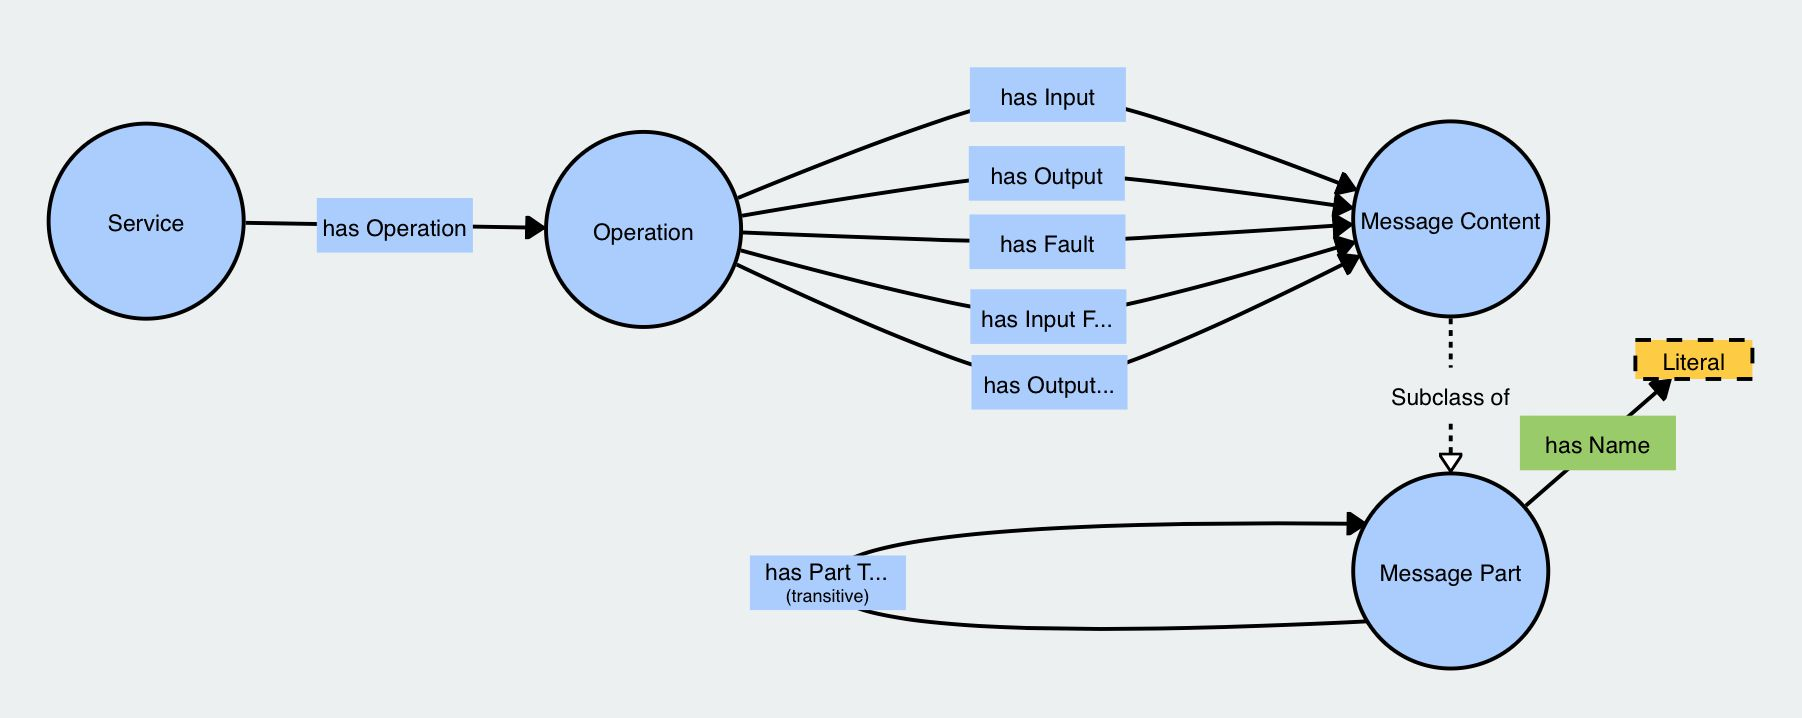
\includegraphics[width=1\textwidth]{resources/chapter-2/msm-visualization.jpg}
	\caption{Visualisasi Ontology Minimal Service Model \parencite{third2017linked}}
	\label{image:msm-visualization}
\end{figure}